\chapter{Viabilidade financeira}
O fato da aplicação ser \textit{\gls{open-source}} restringe a possibilidade de se ganhar dinheiro com venda direta, porém possibilita obtenção de lucro por meio de outras formas, como por exemplo:

\begin{itemize}
   \item \textbf{Utilização do servidor do fornecedor}: Nessa ocasião, a empresa contratante pagará um aluguel mensal para utilizar a aplicação hospedada no servidor do fornecedor.
   \item \textbf{Utilização de servidor próprio}: Utilização da aplicação em um servidor próprio da empresa contratante via pagamento de uma taxa de implementação mais uma de manutenção. Apesar de pagar mais pela implementação em um servidor próprio, a empresa contratante terá o direito de personalizar o produto de acordo com suas preferências nesse método de cobrança.
\end{itemize}

Há ainda a possibilidade de compilação independente do código-fonte da aplicação, por conta da premissa \textit{\gls{open-source}} citada anteriormente. Nesses casos, o fornecedor não se responsabilizará pela prestação de suporte.


Como forma de manter a aplicação, será cobrada uma taxa de R\$10,00 de cada aluno (sendo pago por ele ou pelo mantenedor da instituição de ensino) para que seu acesso à aplicação seja concedido. Desse modo, os custos com hospedagem já estariam cobertos a longo prazo. A Tabela 4 exibe uma previsão orçamentária para o projeto.

\ABNTEXfontereduzida
\begin{table}[htb]
\centering
\caption{Previsão orçamentária mensal do Projeto Turma de Elite}
\begin{tabular}{|p{2.5cm}|c|c|c|c|c|}
   \hline
   \thead{} & \thead{100 alunos}  & \thead{1000 alunos}  & \thead{5000 alunos} & \thead{10000 alunos} & \thead{50000 alunos} \\\hline
   Heroku & R\$127* & R\$506* & R\$1010* & R\$5048* & R\$10096*  \\\hline
    Firebase Hosting & R\$0 & R\$177* & R\$411* & R\$832* & R\$5689* \\\hline
    Firebase Authentication & R\$0 & R\$0 & R\$0 & R\$3029* & R\$18172* \\\hline
    Receita & R\$1000 & R\$10000 & R\$50000 & R\$100000 & R\$500000 \\\hline
    Lucro & R\$873 & R\$9317 & R\$48579 & R\$91091 & R\$466043\\\hline
\end{tabular}
\fonte{Dados do Projeto}
\legend{* - O valor exibido foi aproximado com base na cotação do dólar americano para o dia 08/06/2021 (US\$1 = R\$5,04)}
\end{table}

Com relação aos \textit{\gls{dyno}} do \textit{Heroku} para hospedar a quantidade crescente de acessos concorrentes, a relação obtida foi:
\begin{itemize}
    \item \textbf{100 alunos}: 1 \textit{\gls{dyno}} - \textit{Standard} 1X
    \item \textbf{1000 alunos}: 2 \textit{\glspl{dyno}} - Standard 2X
    \item \textbf{5000 alunos}: 4 \textit{\glspl{dyno}} - Standard 2X
    \item \textbf{10000 alunos}: 4 \textit{\glspl{dyno}} - Performance M
    \item \textbf{50000 alunos}: 2 \textit{\glspl{dyno}} - Performance L
\end{itemize}

A Figura 7 apresenta as relações de preço presentes no website do Heroku.

\begin{figure}[htb]
    \centering
	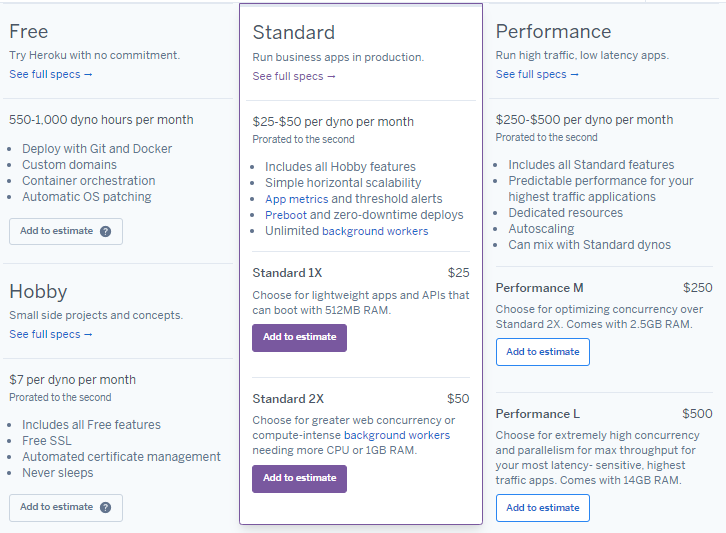
\includegraphics[width=16cm]{imagens/precos-heroku.png}
	\caption{Preço mensal de aluguel dos \textit{\glspl{dyno}} do Heroku}
	\fonte{\cite{heroku:2021}}
\end{figure}


O custo de hospedagem e autenticação variou conforme a quantidade de armazenamento e suporte a acessos simultâneos necessários para atender a quantidade crescente de alunos.